\documentclass{article}

% Import necessary packages
\usepackage[preprint]{neurips_2020}
\usepackage[utf8]{inputenc} % allow utf-8 input
\usepackage[T1]{fontenc}    % use 8-bit T1 fonts
\usepackage{hyperref}       % hyperlinks
\usepackage{url}            % simple URL typesetting
\usepackage{booktabs}       % professional-quality tables
\usepackage{amsfonts}       % blackboard math symbols
\usepackage{nicefrac}       % compact symbols for 1/2, etc.
\usepackage{microtype}      % microtypography

\usepackage{graphicx}       % For importing the pictures
\usepackage{tabularx}
\usepackage{makecell}
\usepackage{float}
\usepackage{lmodern}
\usepackage{subcaption}


\title{COMP47650 – Deep Learning Project Report}

\author{
  Yu Du \\
  \texttt{yu.du2@ucdconnect.ie} \\
}

\date{}


\begin{document}

  \maketitle

  \begin{abstract}

    This article presents the implementation process of an audio genre classification model on the GTZAN dataset, based on the classic Transformer architecture and the Whisper speech recognition framework. To explore improvements in model performance, several structural variants and hyperparameter configurations were compared to identify the optimal setup. The results indicate that, for small datasets, relatively lightweight models are more likely to achieve better classification performance. Under the two structural variants and multiple hyperparameter configurations evaluated in this study, the model achieved performance roughly comparable to human-level accuracy in distinguishing audio genres.

  \end{abstract}

  \section{Introduction}

    With the rapid development of deep learning, the field has evolved from simple perceptrons to modern, complex transformer architectures. Each technological innovation has brought about tremendous changes—whether in academic research, everyday life, or industrial applications. In particular, after Google introduced the transformer architecture in 2017, many companies began actively exploring, improving, and applying it across various domains.

    Among them, OpenAI deserves special mention. It developed one of the most advanced generative AI tools based on transformer architecture —- ChatGPT -— which marked a major breakthrough in traditional language models. Later, OpenAI also applied a transformer-based model called Whisper to speech recognition and achieved excellent performance. This extension is valuable because it enables language models to process not only text but also audio data.
    
    Coincidentally, my assignment also involves audio-type data. Therefore, I decided to attempt modifying and applying one of the most widely used deep learning frameworks -— TensorFlow -— together with the transformer architecture used in Whisper, to complete this project. My goal is to classify music genres in the GTZAN audio dataset.
    
    In this report, I will first analyze the features and limitations of previous models. Then, I will describe in detail the process of building and modifying my own model. Finally, I will summarize the key outcomes of this attempt.


  \section{Related Work}

    As early as 2002, George et al. studied the problem of music genre classification and proposed three features to describe musical characteristics: timbre texture, rhythm, and pitch. Finally, they tested their approach using audio samples collected from CDs, radio, and the internet, achieving an accuracy of 61\%, which was comparable to human classification performance at that time. This suggests that extracting effective audio features can significantly improve classification accuracy.

    More recently, Keoikantse (2024) attempted to use machine learning methods for the same task. His results showed that KNN (with an accuracy of 55\%) outperformed CNN (40\%). He also evaluated the Random Forest method, which further improved the accuracy to an impressive 84\%. These results suggest that using a more complex model is not always better for genre classification. In contrast, lightweight and more randomized models may yield better performance.


  \section{Experimental Setup}

    \subsection{Data Preprocess}

      The GTZAN dataset contains 10 music genres, with 100 WAV-format audio files for each genre (as shown in Figure \ref{fig:shape_preprocess}). Each audio file is approximately 30 seconds in length. After inspecting the audio headers, I found that the files use a 22,050 Hz sampling rate, mono channel, and 16-bit depth.

      Based on these data characteristics, I divided the data preprocessing stage into two steps to handle the GTZAN audio dataset: 

      \begin{itemize}
        \item Data reading
        \item Data conversion
      \end{itemize}

      \begin{figure}[H]
        \centering
        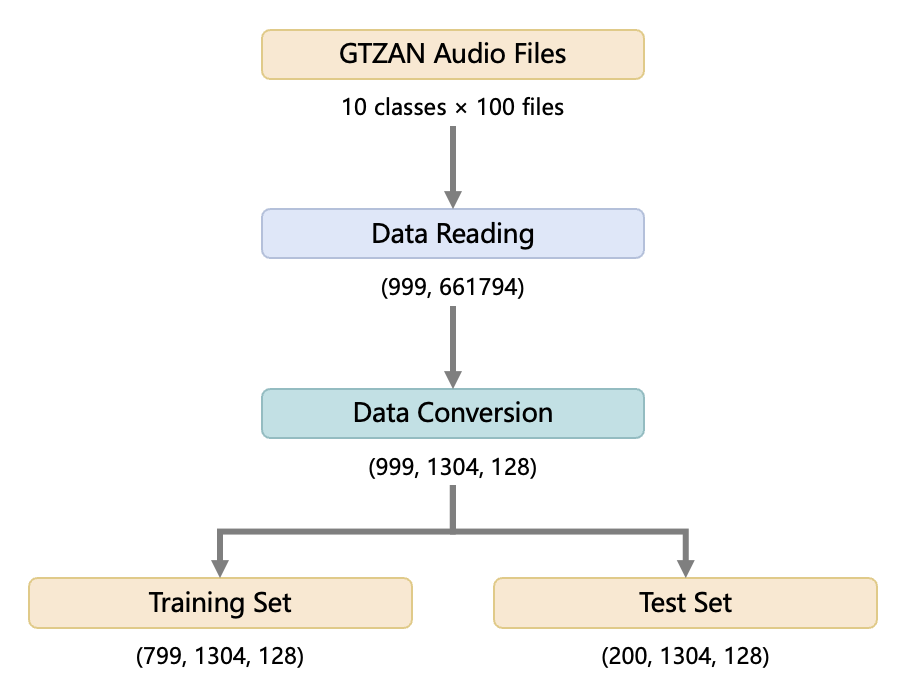
\includegraphics[width=0.5\textwidth]{figs/shape_preprocess.png}
        \caption{Data shape flow chart of each step of data preprocessing.}
        \label{fig:shape_preprocess}
      \end{figure}

      In the data reading step, raw bit strings were extracted from the GTZAN audio files and converted into float32-type TensorFlow tensors (as shown in Figure \ref{fig:shape_preprocess}). The resulting data shape is: 999 samples with 661,794 sample points each, which facilitates the subsequent computation.

      There are two notable points:

      \begin{enumerate}
        \item The audio file No.00054 in the jazz genre is corrupted, so it was excluded from the dataset.
        \item Although each audio clip is about 30 seconds, their lengths are not perfectly aligned. Therefore, I padded them with zeros to match the maximum length among all files.
      \end{enumerate}
      
      During this process, I also implemented a function called data loading with persistence. This function not only reads the audio data and converts the data type, but also saves the processed data as .txt files. This helps avoid repeated data loading and improves efficiency during training and testing.

      In the data conversion step, the raw float32 data are first processed using the Short-Time Fourier Transform (STFT) with a specified frame length and frame shift (also known as frame step), converting the data from the time domain to the frequency domain (i.e., a spectrogram). Next, the spectrogram is transformed using a log-Mel scale, simulating human auditory perception to extract relevant information.

      At this stage, the data shape becomes three-dimensional: 999 samples, 1304 time steps, and 128 Mel bins (as shown in Figure \ref{fig:shape_preprocess}). Then, the 3D tensor is normalized to have zero mean and unit variance, which helps prevent issues such as gradient vanishing or explosion during training. After normalization, data augmentation is applied to improve model generalization. Finally, the data are split into a training set and a test set, using a fixed random seed of 2025 as specified in the assignment. In this stage, I also implemented a data persistence option, consistent with the previous step.

    \subsection{Model Construction}

      \begin{figure}[H]
        \centering
        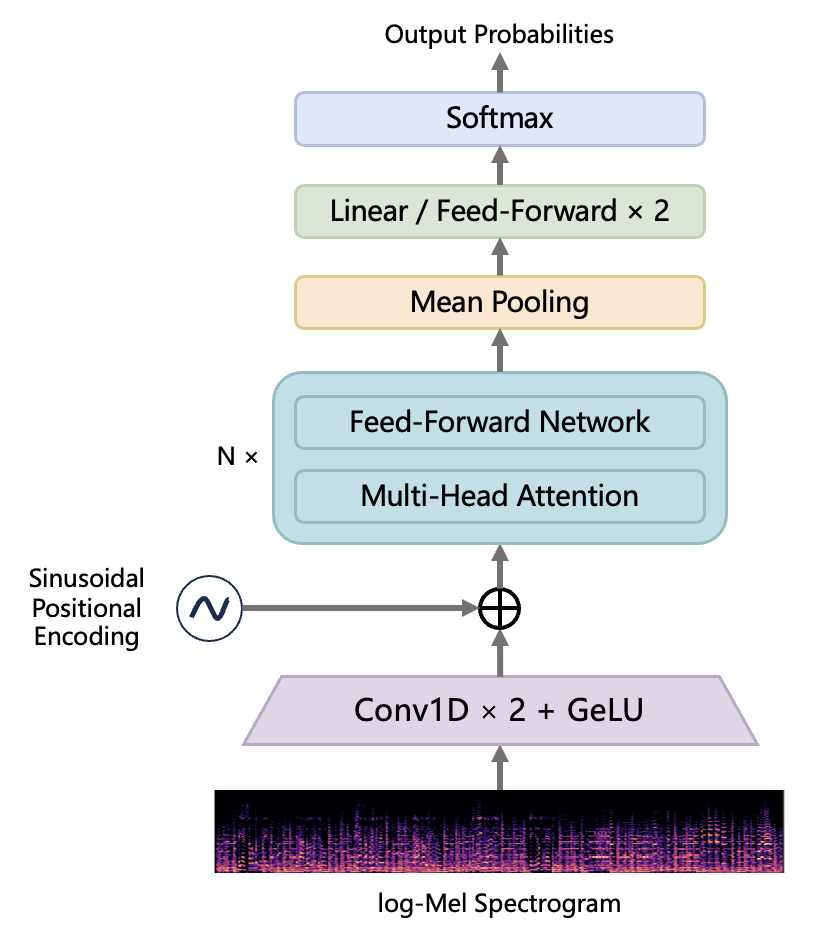
\includegraphics[width=0.4\textwidth]{figs/architecture.png}
        \caption{Complete model architecture.}
        \label{fig:model_architecture}
      \end{figure}

      As shown in Figure \ref{fig:model_architecture}, I divided the complete model into three parts:

      \begin{itemize}
        \item Pre-encoder
        \item Encoder
        \item Audio classifier
      \end{itemize}

      The first part, the pre-encoder, follows the Whisper architecture, consisting of two convolutional layers with GeLU activation, designed to extract spatial features and perform downsampling. After expanding the log-Mel spectrogram, sinusoidal positional encoding is applied to inject temporal information, following the traditional Transformer design using sine and cosine functions. It is worth mentioning that L2 regularization was added to the convolutional layers, as well as to the subsequent feed-forward and linear sublayers, to reduce the risk of overfitting.

      The second part, the encoder, follows the traditional Transformer architecture, which consists of two sub-layers: a feed-forward network and multi-head attention. Since this structure is already well-established and widely used, I did not make any modifications.

      Typically, a standard Transformer also includes a decoder, which plays a crucial role in sequence generation tasks. However, because my task is a multi-class classification problem, the decoder is unnecessary.

      The third part, the audio classifier, includes two alternative designs. The first follows the output structure of the original Transformer, consisting of a linear layer followed by a Softmax function. In the second approach, I replaced the linear layer with two feed-forward layers to allow the model to learn more complex representations.

    \subsection{Experimental Setup}

      Based on the completed model architecture, I conducted the following experiments to examine how different architectural choices affect classification accuracy:

      \begin{table}[H]
        \caption{Architecture vs Hyper-parameter.}
        \label{tbl:arch_hyper_param}
        \centering
        \begin{tabularx}{\textwidth}{clccccc}
          \toprule
           & Classifier
                  & \makecell{Filters \\ Number} 
                  & \makecell{Heads \\ Number} 
                  & \makecell{Feed-Forward \\ Dimension} 
                  & \makecell{Encoders \\ Number} 
                  & \makecell{Hidden \\ Dimension} \\
          \midrule
          (a) & Linear Classifier & 512                       & 8             & 1024                    & 6               & - \\
          (b) & Linear Classifier & 384                       & 8             & 512                     & 4               & - \\
          (c) & FFN Classifier    & 384                       & 8             & 512                     & 6               & 128 \\
          (d) & FFN Classifier    & 256                       & 8             & 1024                    & 3               & 128 \\
          \bottomrule
        \end{tabularx}
      \end{table}

      In the overall model architecture, by slightly adjusting the local structure and parameters —- including the number of filters in the pre-encoder sublayer, the number of heads and feed-forward dimensions in the encoder, the number of encoder layers, and the hidden dimensions of the classifier—we can compare which architectural combination yields the highest accuracy.

      In these four experiments, I used the configuration with a linear classifier, 512 filters, 8 attention heads, a 1024-dimensional feed-forward network, and 6 encoder layers as the baseline model, since this setup exactly follows the configuration of the basic version of the Whisper model. In practice, I continuously adjusted parts of the structure and changed parameter settings as part of the experimental design, especially when the current results were not satisfactory.


  \section{Results}

    Based on these four configurations, we obtained the following four models with their corresponding highest accuracies:

    \begin{table}[H]
      \caption{The highest accuracy.}
      \label{tbl:highest_acc}
      \centering
      \begin{tabular}{lcc}
        \toprule
        & Training Set(\%) & Validation Set(\%) \\
        \midrule
        (a) & 77.6 & 54.0 \\
        (b) & 76.5 & 60.5 \\
        (c) & 77.4 & 51.0 \\
        (d) & 79.9 & 60.0 \\
        \bottomrule
      \end{tabular}
    \end{table}
    
    From the accuracy results, the models performed consistently well on the training set. However, on the validation set, the performance was less stable, with some fluctuations. In particular, the models with configurations (a) and (c) had heavier overall structures compared to (b) and (d), as they each contained six encoder layers. Between (a) and (c), the accuracy of configuration (c) was even lower than that of (a), suggesting that increasing model complexity does not always lead to better results —- especially considering that the dataset only contains about 1000 audio samples.

    \begin{figure}[H]
      \centering
      \begin{subfigure}[b]{0.45\textwidth}
        \centering
        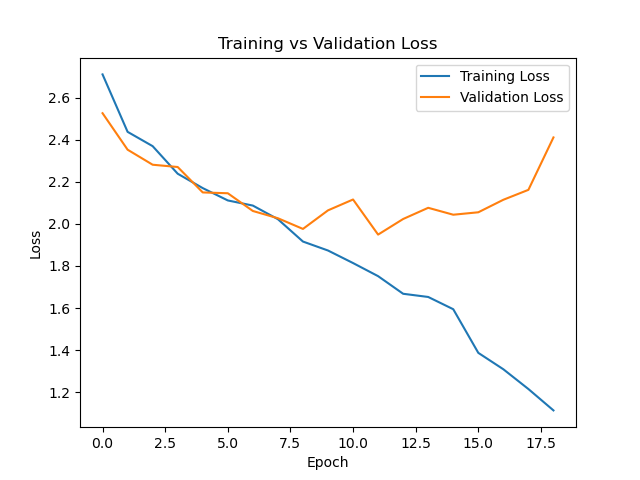
\includegraphics[width=\textwidth]{figs/loss_curve_1.png}
        \caption{}
        \label{fig:loss_curve_1}
      \end{subfigure}
      \hfill
      \begin{subfigure}[b]{0.45\textwidth}
        \centering
        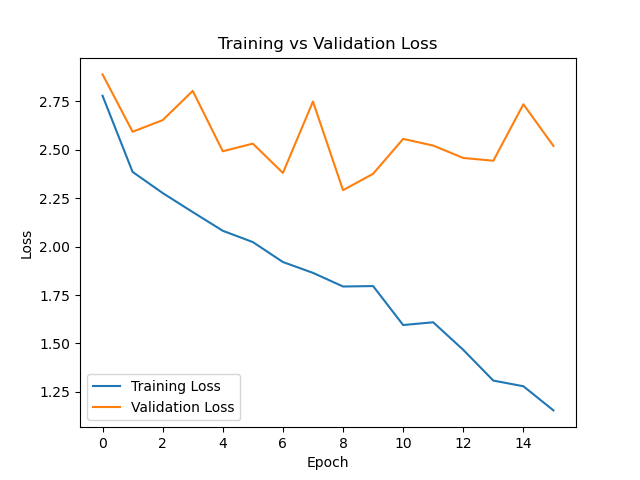
\includegraphics[width=\textwidth]{figs/loss_curve_2.png}
        \caption{}
        \label{fig:loss_curve_2}
      \end{subfigure}
      
      \vspace{0.5em}
      
      \begin{subfigure}[b]{0.45\textwidth}
        \centering
        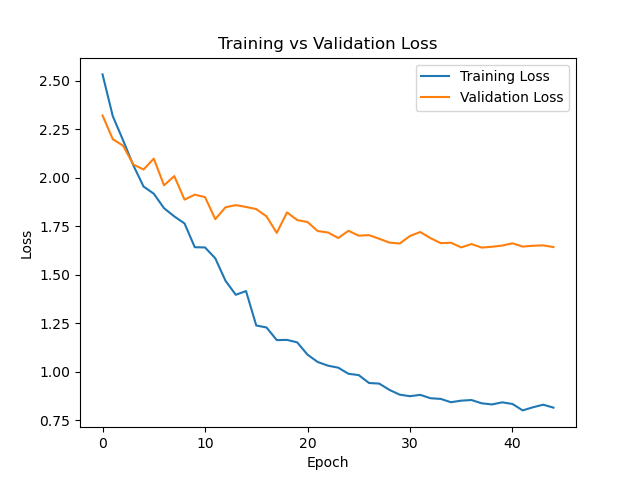
\includegraphics[width=\textwidth]{figs/loss_curve_3.png}
        \caption{}
        \label{fig:loss_curve_3}
      \end{subfigure}
      \hfill
      \begin{subfigure}[b]{0.45\textwidth}
        \centering
        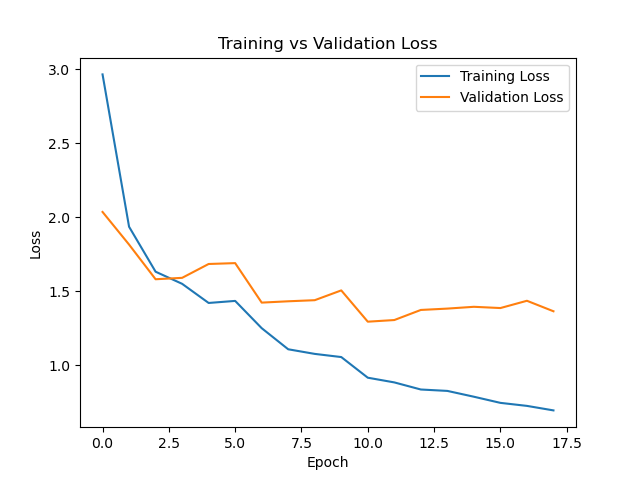
\includegraphics[width=\textwidth]{figs/loss_curve_4.png}
        \caption{}
        \label{fig:loss_curve_4}
      \end{subfigure}
    
      \caption{Loss curves for four experiments}
      \label{fig:loss_curve}
    \end{figure}

    An analysis of the loss curves from the four experiments reveals notable patterns. In model (a), the training and validation loss curves begin to diverge after the 8th epoch—the training loss continues to decrease steadily, while the validation loss starts to increase, indicating overfitting. As the model complexity is reduced in model (b), the validation loss no longer increases but shows minor oscillations and signs of non-convergence. In models (c) and (d), which use a two-layer feed-forward classifier, convergence is significantly improved. However, these models still suffer from limited generalization ability, suggesting room for further optimization.


  \section{Conclusion And Future Work}

    In this project, we explored the task of audio genre classification on the GTZAN dataset by implementing a model based on the Transformer architecture and the Whisper speech recognition framework. During the experiments, we found that under a limited dataset, relatively lightweight model structures tended to achieve better performance. When the model reached its best state—with an accuracy of 60\% -— its performance was roughly comparable to the human ability to distinguish between audio genres.

    Although this project was constrained by time and other factors, and the hyperparameter tuning was not fully optimized, the model was still able to meet the task requirements. In future work, I plan to continue addressing the remaining issues, particularly by conducting further hyperparameter optimization and exploring potential improvements to the model architecture. The goal is to achieve a more stable and accurate model capable of higher classification performance.


  \section*{References}

    {\small

      [1] Mogonediwa, K. (2024). \textit{Music genre classification: Training an AI model}. arXiv preprint arXiv:2405.15096. Retrieved from \url{https://arxiv.org/abs/2405.15096}.

      [2] Tzanetakis, G., \& Cook, P. (2002). \textit{Musical genre classification of audio signals}. \textit{IEEE Transactions on Speech and Audio Processing}, 10(5), 293--302. \url{https://doi.org/10.1109/TSA.2002.800560}.

      [3] Vaswani, A., Shazeer, N., Parmar, N., Uszkoreit, J., Jones, L., Gomez, A. N., Kaiser, {\L}., \& Polosukhin, I. (2017). \textit{Attention is all you need}. In \textit{Advances in Neural Information Processing Systems} (Vol. 30, pp. 5998--6008). Curran Associates, Inc. Retrieved from \url{https://papers.nips.cc/paper/7181-attention-is-all-you-need.pdf}.

      [4] Radford, A., Kim, J. W., Xu, T., Brockman, G., McLeavey, C., \& Sutskever, I. (2023). \textit{Robust speech recognition via large-scale weak supervision}. In \textit{Proceedings of the 40th International Conference on Machine Learning} (Vol. 202, pp. 28492--28518). PMLR. Retrieved from \url{https://proceedings.mlr.press/v202/radford23a.html}.

    }


\end{document}

